We can interpret the biased regularization in the following way. Let $w_{N+1} = w_{N+1}''+\sum\limits{\beta _kw'_k}$ (See Figure \ref{fig:combine}). Therefore, we have:
\begin{equation*}
w_{N+1}\phi(x)=w_{N+1}''\phi(x)+\sum\limits{\beta _kw'_k\phi(x)}
\end{equation*}

\begin{figure}
\centering
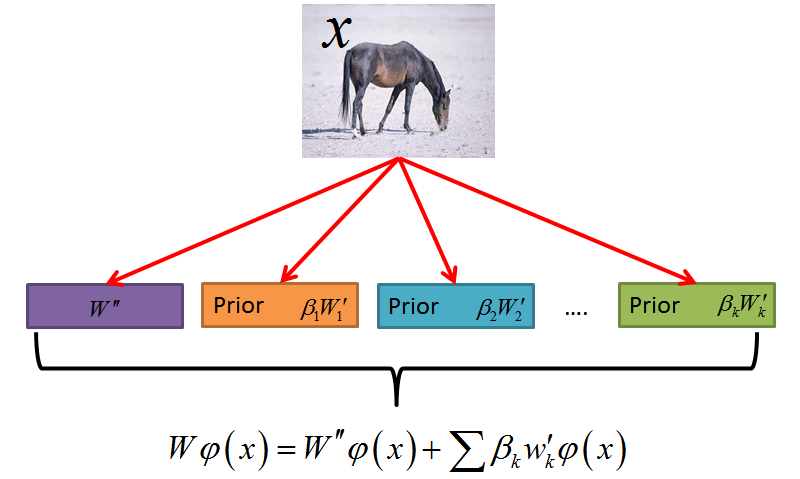
\includegraphics[scale=0.25]{fig/combine.png}
\caption{The final decision function value of a binary SVM can be get by combining the prior and empirical knowledge.}\label{fig:combine}
\end{figure}
Here, we call $\beta$ the transfer parameter. For any fixed value of $\beta$, regularizing $w_n$ is equivalent to regularize $w_{N+1}''$, i.e. $(w_{N+1}-\sum\limits{\beta _kw'_k})$. The decision of each binary SVM model is made by combining the decision from target task $w_{N+1}''\phi(x)$ and source hypotheses $w'_k\phi(x)$ controlled by the transfer parameter. The amount of transfered knowledge has a positive correlation to the value of $\beta$.